% Options for packages loaded elsewhere
\PassOptionsToPackage{unicode}{hyperref}
\PassOptionsToPackage{hyphens}{url}
\PassOptionsToPackage{space}{xeCJK}
\documentclass[
]{article}
\usepackage{xcolor}
\usepackage[margin=24mm]{geometry}
\usepackage{amsmath,amssymb}
\setcounter{secnumdepth}{-\maxdimen} % remove section numbering
\usepackage{iftex}
\ifPDFTeX
  \usepackage[T1]{fontenc}
  \usepackage[utf8]{inputenc}
  \usepackage{textcomp} % provide euro and other symbols
\else % if luatex or xetex
  \usepackage{unicode-math} % this also loads fontspec
  \defaultfontfeatures{Scale=MatchLowercase}
  \defaultfontfeatures[\rmfamily]{Ligatures=TeX,Scale=1}
\fi
\usepackage{lmodern}
\ifPDFTeX\else
  % xetex/luatex font selection
  \setmainfont[]{HaranoAjiMincho-Regular.otf}
  \setmonofont[]{DejaVuSansMono.ttf}
  \ifXeTeX
    \usepackage{xeCJK}
    \setCJKmainfont[]{HaranoAjiMincho-Regular.otf}
  \fi
  \ifLuaTeX
    \usepackage[]{luatexja-fontspec}
    \setmainjfont[]{HaranoAjiMincho-Regular.otf}
  \fi
\fi
% Use upquote if available, for straight quotes in verbatim environments
\IfFileExists{upquote.sty}{\usepackage{upquote}}{}
\IfFileExists{microtype.sty}{% use microtype if available
  \usepackage[]{microtype}
  \UseMicrotypeSet[protrusion]{basicmath} % disable protrusion for tt fonts
}{}
\makeatletter
\@ifundefined{KOMAClassName}{% if non-KOMA class
  \IfFileExists{parskip.sty}{%
    \usepackage{parskip}
  }{% else
    \setlength{\parindent}{0pt}
    \setlength{\parskip}{6pt plus 2pt minus 1pt}}
}{% if KOMA class
  \KOMAoptions{parskip=half}}
\makeatother
\usepackage{color}
\usepackage{fancyvrb}
\newcommand{\VerbBar}{|}
\newcommand{\VERB}{\Verb[commandchars=\\\{\}]}
\DefineVerbatimEnvironment{Highlighting}{Verbatim}{commandchars=\\\{\}}
% Add ',fontsize=\small' for more characters per line
\newenvironment{Shaded}{}{}
\newcommand{\AlertTok}[1]{\textcolor[rgb]{1.00,0.00,0.00}{\textbf{#1}}}
\newcommand{\AnnotationTok}[1]{\textcolor[rgb]{0.38,0.63,0.69}{\textbf{\textit{#1}}}}
\newcommand{\AttributeTok}[1]{\textcolor[rgb]{0.49,0.56,0.16}{#1}}
\newcommand{\BaseNTok}[1]{\textcolor[rgb]{0.25,0.63,0.44}{#1}}
\newcommand{\BuiltInTok}[1]{\textcolor[rgb]{0.00,0.50,0.00}{#1}}
\newcommand{\CharTok}[1]{\textcolor[rgb]{0.25,0.44,0.63}{#1}}
\newcommand{\CommentTok}[1]{\textcolor[rgb]{0.38,0.63,0.69}{\textit{#1}}}
\newcommand{\CommentVarTok}[1]{\textcolor[rgb]{0.38,0.63,0.69}{\textbf{\textit{#1}}}}
\newcommand{\ConstantTok}[1]{\textcolor[rgb]{0.53,0.00,0.00}{#1}}
\newcommand{\ControlFlowTok}[1]{\textcolor[rgb]{0.00,0.44,0.13}{\textbf{#1}}}
\newcommand{\DataTypeTok}[1]{\textcolor[rgb]{0.56,0.13,0.00}{#1}}
\newcommand{\DecValTok}[1]{\textcolor[rgb]{0.25,0.63,0.44}{#1}}
\newcommand{\DocumentationTok}[1]{\textcolor[rgb]{0.73,0.13,0.13}{\textit{#1}}}
\newcommand{\ErrorTok}[1]{\textcolor[rgb]{1.00,0.00,0.00}{\textbf{#1}}}
\newcommand{\ExtensionTok}[1]{#1}
\newcommand{\FloatTok}[1]{\textcolor[rgb]{0.25,0.63,0.44}{#1}}
\newcommand{\FunctionTok}[1]{\textcolor[rgb]{0.02,0.16,0.49}{#1}}
\newcommand{\ImportTok}[1]{\textcolor[rgb]{0.00,0.50,0.00}{\textbf{#1}}}
\newcommand{\InformationTok}[1]{\textcolor[rgb]{0.38,0.63,0.69}{\textbf{\textit{#1}}}}
\newcommand{\KeywordTok}[1]{\textcolor[rgb]{0.00,0.44,0.13}{\textbf{#1}}}
\newcommand{\NormalTok}[1]{#1}
\newcommand{\OperatorTok}[1]{\textcolor[rgb]{0.40,0.40,0.40}{#1}}
\newcommand{\OtherTok}[1]{\textcolor[rgb]{0.00,0.44,0.13}{#1}}
\newcommand{\PreprocessorTok}[1]{\textcolor[rgb]{0.74,0.48,0.00}{#1}}
\newcommand{\RegionMarkerTok}[1]{#1}
\newcommand{\SpecialCharTok}[1]{\textcolor[rgb]{0.25,0.44,0.63}{#1}}
\newcommand{\SpecialStringTok}[1]{\textcolor[rgb]{0.73,0.40,0.53}{#1}}
\newcommand{\StringTok}[1]{\textcolor[rgb]{0.25,0.44,0.63}{#1}}
\newcommand{\VariableTok}[1]{\textcolor[rgb]{0.10,0.09,0.49}{#1}}
\newcommand{\VerbatimStringTok}[1]{\textcolor[rgb]{0.25,0.44,0.63}{#1}}
\newcommand{\WarningTok}[1]{\textcolor[rgb]{0.38,0.63,0.69}{\textbf{\textit{#1}}}}
\usepackage{longtable,booktabs,array}
\newcounter{none} % for unnumbered tables
\usepackage{calc} % for calculating minipage widths
% Correct order of tables after \paragraph or \subparagraph
\usepackage{etoolbox}
\makeatletter
\patchcmd\longtable{\par}{\if@noskipsec\mbox{}\fi\par}{}{}
\makeatother
% Allow footnotes in longtable head/foot
\IfFileExists{footnotehyper.sty}{\usepackage{footnotehyper}}{\usepackage{footnote}}
\makesavenoteenv{longtable}
\usepackage{graphicx}
\makeatletter
\newsavebox\pandoc@box
\newcommand*\pandocbounded[1]{% scales image to fit in text height/width
  \sbox\pandoc@box{#1}%
  \Gscale@div\@tempa{\textheight}{\dimexpr\ht\pandoc@box+\dp\pandoc@box\relax}%
  \Gscale@div\@tempb{\linewidth}{\wd\pandoc@box}%
  \ifdim\@tempb\p@<\@tempa\p@\let\@tempa\@tempb\fi% select the smaller of both
  \ifdim\@tempa\p@<\p@\scalebox{\@tempa}{\usebox\pandoc@box}%
  \else\usebox{\pandoc@box}%
  \fi%
}
% Set default figure placement to htbp
\def\fps@figure{htbp}
\makeatother
\setlength{\emergencystretch}{3em} % prevent overfull lines
\providecommand{\tightlist}{%
  \setlength{\itemsep}{0pt}\setlength{\parskip}{0pt}}
\usepackage{bookmark}
\IfFileExists{xurl.sty}{\usepackage{xurl}}{} % add URL line breaks if available
\urlstyle{same}
\hypersetup{
  hidelinks,
  pdfcreator={LaTeX via pandoc}}

\author{}
\date{}

\begin{document}

\section{フェルミオン的逆相核による完全反射写像の干渉構成}\label{ux30d5ux30a7ux30ebux30dfux30aaux30f3ux7684ux9006ux76f8ux6838ux306bux3088ux308bux5b8cux5168ux53cdux5c04ux5199ux50cfux306eux5e72ux6e09ux69cbux6210}

\textbf{副題:}
交換二経路の干渉消去と相対位相節からの方向反転の数値構成実験\\
\textbf{日付:} 2026-07-10\\
\textbf{著者:} 木原 範昭\\
\textbf{位置づけ:} 追加論文・数値実験実行稿\\
\textbf{Version DOI:} 10.5281/zenodo.21295480\\
\textbf{Concept DOI:} 10.5281/zenodo.21295479

\begin{center}\rule{0.5\linewidth}{0.5pt}\end{center}

\subsection{要旨}\label{ux8981ux65e8}

本稿では、先行する「背景空間を仮定しない閉じた位相系におけるフェルミオン的二局所波の完全弾性反射の構成実験」において、有限解像度相互作用セル内の構成規則として与えていた方向反転写像を、外部条件分岐なしに、フェルミオン的内部逆相核と交換二経路の波動干渉から生成できるかを実行した。

局所波 \texttt{A,B} は、空間位相 \texttt{χ}、時間位相
\texttt{τ}、内部識別位相
\texttt{η}、代表振幅、およびフェルミオン的逆相核を持つ。二局所波の相互作用に対して、直接経路
\texttt{P\_A(1)P\_B(2)} と交換経路 \texttt{P\_A(2)P\_B(1)}
を構成し、内部核位相差 \texttt{Δ\_F}
を交換経路の相対位相として転写する。

一般化された二経路合成

\[\Psi_{\Delta}(1,2)
=
\frac{1}{\sqrt2}
\left[
P_A(1)P_B(2)
+
e^{i\Delta_F}P_A(2)P_B(1)
\right]\]

を用いると、完全重なり点 \texttt{1=2} において、\texttt{Δ\_F=π}
では二経路が完全に干渉消去される。

\[\Psi_{\pi}(1,1)=0\]

本稿では、左側から入射する単一局在波束を初期状態とし、外部方向反転命令、鏡像初期条件、反射境界条件を用いずに時間発展させた。相互作用領域では、直接経路と交換経路を偶・奇干渉チャンネルへ分解し、内部逆相核の位相差のみを奇チャンネルへ転写して再合成した。

実行結果では、\texttt{Δ\_F=0} で反射率
\texttt{1.8261693781071190e-19}、通過率
\texttt{1.0000000000000002}、\texttt{Δ\_F=π/2} で反射率・通過率ともに
\texttt{0.5}、\texttt{Δ\_F=π} で反射率
\texttt{1.0000000000000002}、通過率 \texttt{1.7939211291143336e-19}
が得られた。位相掃引全体で \texttt{R(Δ\_F)=sin\^{}2(Δ\_F/2)},
\texttt{T(Δ\_F)=cos\^{}2(Δ\_F/2)} が最大誤差
\texttt{5.551115123125783e-16} で再現され、ノルム最大誤差は
\texttt{6.661338147750939e-16} であった。局所交換干渉写像は
\texttt{U(π)\^{}2} 相対誤差
\texttt{4.8214412843789535e-11}、\texttt{U(Δ\_F)U(-Δ\_F)} 最大相対誤差
\texttt{1.4547631339456792e-16}
で可逆性を満たした。補償付き二乗閉鎖の最大残差は
\texttt{1.2143074258005e-17} であった。内部識別振動 \texttt{m\_A,m\_B}
は読出し相関により保存された。

\textbf{キーワード:}
フェルミオン的逆相核、交換干渉、相対位相節、完全反射、内部観測、有限解像度セル、無名等振幅複合波

\begin{center}\rule{0.5\linewidth}{0.5pt}\end{center}

\subsection{1. 序論}\label{1-ux5e8fux8ad6}

前論文では、背景空間を先験的に仮定しない閉じた位相系において、識別可能な二つのフェルミオン的局所波が、有限解像度相互作用セル内で完全弾性反射する保存写像を構成した。

前論文の写像は、相互作用セル内で

\[q_A\mapsto -q_A,
\qquad
q_B\mapsto -q_B\]

を適用する構成規則として与えられていた。

この規則は、局在、識別振動、観測、閉鎖、可逆性と両立することが確認された。本稿では、方向反転そのものを、外部命令ではなく、波の干渉過程から内部生成する機構として実行した。

本稿の問いは次である。

\begin{quote}
フェルミオン的内部逆相核が、二局所波の交換二経路間に相対位相 \texttt{π}
を自動的に与え、その干渉によって通過成分を消去し、完全反射に相当する方向反転出力を生成できるか。
\end{quote}

本稿では、外部条件分岐

\begin{Shaded}
\begin{Highlighting}[]
\NormalTok{if fermion:}
\NormalTok{    reverse\_direction()}
\end{Highlighting}
\end{Shaded}

を用いない。

内部位相、局在波重なり、交換経路、干渉再合成、および内部観測のみを用いて反射出力を得る。

\begin{center}\rule{0.5\linewidth}{0.5pt}\end{center}

\subsection{2.
本稿で主張しないこと}\label{2-ux672cux7a3fux3067ux4e3bux5f35ux3057ux306aux3044ux3053ux3068}

本稿は、以下を主張しない。

{\def\LTcaptype{none} % do not increment counter
\begin{longtable}[]{@{}ll@{}}
\toprule\noalign{}
主張しないこと & 理由 \\
\midrule\noalign{}
\endhead
\bottomrule\noalign{}
\endlastfoot
標準的なフェルミ粒子散乱の導出 &
標準ハミルトニアン、S行列、散乱断面積を用いない \\
パウリ排他原理そのものの導出 &
フェルミオン的とは内部逆相核を持つ作業的分類である \\
節形成だけから一般に反射が必然であること &
通過流抑制と反射出力生成は数値実験で確認する \\
実在粒子の交換相互作用の定量予言 &
本稿は位相波モデル内の構成可能性実験である \\
外部時空における粒子軌道の再現 & \texttt{χ,τ}
は閉じた位相系内の読出し変数である \\
\end{longtable}
}

本稿の主張は、内部逆相核から交換干渉符号を生成し、その干渉により反射写像を内部生成する数値構成である。

\begin{center}\rule{0.5\linewidth}{0.5pt}\end{center}

\subsection{3. 基本構造}\label{3-ux57faux672cux69cbux9020}

\subsubsection{3.1 局所波}\label{31-ux5c40ux6240ux6ce2}

局所波 \texttt{P} を、空間位相 \texttt{χ}、時間位相
\texttt{τ}、内部識別位相 \texttt{η} 上で次のように表す。

\[P(\chi,\tau,\eta)
=
A_P
S_{N_{h,\chi}^{P}}(\chi-\chi_P)
S_{N_{h,\tau}^{P}}(\tau-\tau_P)
e^{im_P\eta}
e^{i\phi_P}\]

ここで、

\begin{itemize}
\tightlist
\item
  \texttt{A\_P} は代表振幅
\item
  \texttt{S\_\{N\_h\}} は正規化等振幅奇数倍音局在波
\item
  \texttt{m\_P} は内部識別振動モード
\item
  \texttt{φ\_P} は局所位相
\end{itemize}

である。

\subsubsection{3.2
正規化等振幅奇数倍音局在波}\label{32-ux6b63ux898fux5316ux7b49ux632fux5e45ux5947ux6570ux500dux97f3ux5c40ux5728ux6ce2}

\[S_{N_h}(u)
=
\frac{1}{K}
\sum_{m=0}^{K-1}
\cos((2m+1)u),
\qquad
N_h=2K-1\]

閉形式は、

\[S_{N_h}(u)
=
\frac{\sin((N_h+1)u)}{(N_h+1)\sin u}\]

である。

\subsubsection{3.3
フェルミオン的内部逆相核}\label{33-ux30d5ux30a7ux30ebux30dfux30aaux30f3ux7684ux5185ux90e8ux9006ux76f8ux6838}

二成分内部核を、

\[F_P
=
\frac{1}{\sqrt2}
\left(
e^{i\theta_{P,1}},
e^{i\theta_{P,2}}
\right)\]

とし、内部位相差を、

\[\Delta_F
=
\theta_{P,2}-\theta_{P,1}\]

とする。

純粋フェルミオン的逆相核は、

\[\Delta_F=\pi\]

である。

\begin{center}\rule{0.5\linewidth}{0.5pt}\end{center}

\subsection{4.
直接経路と交換経路}\label{4-ux76f4ux63a5ux7d4cux8defux3068ux4ea4ux63dbux7d4cux8def}

局所波 \texttt{A,B} の全引数を、

\[1=(\chi_1,\tau_1,\eta_1),
\qquad
2=(\chi_2,\tau_2,\eta_2)\]

と書く。

直接経路を、

\[\Psi_{\mathrm{direct}}(1,2)
=
P_A(1)P_B(2)\]

交換経路を、

\[\Psi_{\mathrm{exchange}}(1,2)
=
P_A(2)P_B(1)\]

とする。

内部逆相核を交換経路の相対位相として転写した合成波を、

\[\Psi_{\Delta}(1,2)
=
\frac{1}{\sqrt2}
\left[
\Psi_{\mathrm{direct}}(1,2)
+
e^{i\Delta_F}
\Psi_{\mathrm{exchange}}(1,2)
\right]\]

と定義する。

ここで、演算の選択は外部判断ではない。内部位相差 \texttt{Δ\_F}
が、交換経路の干渉位相を直接決める。

\begin{center}\rule{0.5\linewidth}{0.5pt}\end{center}

\subsection{5.
重なり点における節形成}\label{5-ux91cdux306aux308aux70b9ux306bux304aux3051ux308bux7bc0ux5f62ux6210}

完全重なり点 \texttt{1=2} では、直接経路と交換経路は同じ振幅を持つ。

\[\Psi_{\mathrm{direct}}(1,1)
=
\Psi_{\mathrm{exchange}}(1,1)\]

したがって、

\[\Psi_{\Delta}(1,1)
=
\frac{P_A(1)P_B(1)}{\sqrt2}
\left(1+e^{i\Delta_F}\right)\]

となる。

\subsubsection{5.1 同相核}\label{51-ux540cux76f8ux6838}

\[\Delta_F=0\]

なら、

\[1+e^{i\Delta_F}=2\]

であり、重なり成分は残る。

\subsubsection{5.2 逆相核}\label{52-ux9006ux76f8ux6838}

\[\Delta_F=\pi\]

なら、

\[1+e^{i\pi}=0\]

であり、

\[\Psi_{\pi}(1,1)=0\]

となる。

このゼロは、外部遮蔽やポテンシャル障壁ではなく、二つの交換経路の完全干渉消去による節である。

\begin{center}\rule{0.5\linewidth}{0.5pt}\end{center}

\subsection{6.
相対位相と交換反対称性}\label{6-ux76f8ux5bfeux4f4dux76f8ux3068ux4ea4ux63dbux53cdux5bfeux79f0ux6027}

二局所波の相対空間位相を、

\[\rho=\chi_A-\chi_B\]

とする。

粒子交換は、

\[A\leftrightarrow B\]

に対応し、

\[\rho\mapsto-\rho\]

となる。

交換反対称性が相対位相チャンネルに現れる場合、

\[\Psi_F(-\rho)=-\Psi_F(\rho)\]

であるため、

\[\Psi_F(0)=0\]

となる。

この節が、\texttt{ρ\textless{}0} から \texttt{ρ\textgreater{}0}
への通過流を遮断するかを数値的に確認する。

\begin{center}\rule{0.5\linewidth}{0.5pt}\end{center}

\subsection{7.
通過流と反射流}\label{7-ux901aux904eux6d41ux3068ux53cdux5c04ux6d41}

相対位相方向の波動流を作業的に、

\[J_\rho
=
\operatorname{Im}
\left(
\Psi^*
\frac{\partial\Psi}{\partial\rho}
\right)\]

と定義する。

本稿では、この量を標準量子力学の確率流と同一視しない。相対位相方向の複素波形流を評価するための数値指標として用いる。

フェルミオン的逆相条件で、

\[\Psi_F(0)=0\]

かつ、

\[J_\rho(0)=0\]

となり、反対側へ抜ける通過成分が消失するかを調べる。

\begin{center}\rule{0.5\linewidth}{0.5pt}\end{center}

\subsection{8.
干渉による方向反転の生成写像}\label{8-ux5e72ux6e09ux306bux3088ux308bux65b9ux5411ux53cdux8ee2ux306eux751fux6210ux5199ux50cf}

方向成分を、

\[\mathbf a
=
\begin{pmatrix}
a_+\\
a_-
\end{pmatrix}\]

とする。

対称・反対称チャンネルへの変換を、

\[H
=
\frac{1}{\sqrt2}
\begin{pmatrix}
1&1\\
1&-1
\end{pmatrix}\]

で表す。

交換二経路間の内部位相差を反対称チャンネルへ与えると、

\[U(\Delta_F)
=
H
\begin{pmatrix}
1&0\\
0&e^{i\Delta_F}
\end{pmatrix}
H\]

となる。

\texttt{Δ\_F=π} では、

\[U(\pi)
=
\begin{pmatrix}
0&1\\
1&0
\end{pmatrix}\]

であり、

\[|+\rangle\leftrightarrow|-\rangle\]

が得られる。

本稿では、反射率と通過率を結果値として直接代入するのではなく、片側入射波形に対して局所的な偶奇分解、内部位相転写、再合成を作用させ、最終波形から同じ出力が読出されるかを確認する。

\begin{center}\rule{0.5\linewidth}{0.5pt}\end{center}

\subsection{9.
数値実験の実行}\label{9-ux6570ux5024ux5b9fux9a13ux306eux5b9fux884c}

\subsubsection{9.1 基本条件}\label{91-ux57faux672cux6761ux4ef6}

{\def\LTcaptype{none} % do not increment counter
\begin{longtable}[]{@{}lrl@{}}
\toprule\noalign{}
量 & 基本値 & 意味 \\
\midrule\noalign{}
\endhead
\bottomrule\noalign{}
\endlastfoot
\texttt{A\_A,A\_B} & \texttt{1,1} & 代表振幅 \\
\texttt{N\_\{h,χ\}\^{}A,N\_\{h,χ\}\^{}B} & \texttt{99,99} &
空間局在次数 \\
\texttt{N\_\{h,τ\}\^{}A,N\_\{h,τ\}\^{}B} & \texttt{99,99} &
時間局在次数 \\
\texttt{χ\_A(0),χ\_B(0)} & \texttt{-0.2,+0.2} & 初期空間位相 \\
\texttt{q\_A(0),q\_B(0)} & 使用しない & 外部方向反転命令を排除 \\
\texttt{τ\_A(0),τ\_B(0)} & \texttt{-0.2,-0.2} & 初期時間位相 \\
\texttt{m\_A,m\_B} & \texttt{1,2} & 識別振動モード \\
\texttt{Δ\_F} & \texttt{0} から \texttt{π} & 内部核位相差 \\
片側入射波束中心 & \texttt{ρ=-40} & 左側から原点へ向かう単一入射波束 \\
片側入射波数 & \texttt{k\_0=5.0} & 入射方向の位相流 \\
相互作用窓 & ` & ρ \\
\end{longtable}
}

\subsubsection{9.2 実験群}\label{92-ux5b9fux9a13ux7fa4}

{\def\LTcaptype{none} % do not increment counter
\begin{longtable}[]{@{}rll@{}}
\toprule\noalign{}
No. & 実験 & 目的 \\
\midrule\noalign{}
\endhead
\bottomrule\noalign{}
\endlastfoot
1 & 片側入射散乱 & 鏡像初期条件なしに \texttt{R,T} が出るか \\
2 & 局所写像位相掃引 & \texttt{R=sin\^{}2(Δ\_F/2)},
\texttt{T=cos\^{}2(Δ\_F/2)} が再現されるか \\
3 & 交換干渉位相掃引 & \texttt{Δ\_F=0} から \texttt{π}
まで節深さが解析式通り変化するか \\
4 & 逆相核 & \texttt{Δ\_F=π} で完全重なり対角の振幅が消えるか \\
5 & 交換経路除去 & 交換経路なしでは節形成が消えるか \\
6 & 識別振動読出し & \texttt{m\_A,m\_B} が保存されるか \\
7 & 可逆性 & \texttt{U(π)\^{}2≈I} および \texttt{U(Δ\_F)U(-Δ\_F)≈I}
が成り立つか \\
8 & 補償付き二乗閉鎖 & 主要段階で \texttt{x\_n,\ ix\_n}
補償対の二乗閉鎖が保たれるか \\
9 & AB/C セル差し替え & 前回 AB/C シミュレーションのセル内 \texttt{q}
反転を局所交換干渉写像へ置換できるか \\
\end{longtable}
}

実行スクリプトは次である。

\begin{Shaded}
\begin{Highlighting}[]
\NormalTok{run\_fermionic\_interference\_reflection\_v1.py}
\end{Highlighting}
\end{Shaded}

出力先は次である。

\begin{Shaded}
\begin{Highlighting}[]
\NormalTok{fermionic\_interference\_reflection\_result\_v1/}
\end{Highlighting}
\end{Shaded}

\begin{center}\rule{0.5\linewidth}{0.5pt}\end{center}

\subsection{10. 実行結果}\label{10-ux5b9fux884cux7d50ux679c}

\subsubsection{10.1 全体判定}\label{101-ux5168ux4f53ux5224ux5b9a}

{\def\LTcaptype{none} % do not increment counter
\begin{longtable}[]{@{}lr@{}}
\toprule\noalign{}
項目 & 結果 \\
\midrule\noalign{}
\endhead
\bottomrule\noalign{}
\endlastfoot
外部 \texttt{q} 反転代入 & \texttt{false} \\
片側入射初期条件 & \texttt{true} \\
\texttt{Delta\_F=0} で通過 & \texttt{true} \\
\texttt{Delta\_F=pi/2} で半反射 & \texttt{true} \\
\texttt{Delta\_F=pi} で完全反射 & \texttt{true} \\
局所写像位相掃引が期待式と一致 & \texttt{true} \\
局所写像ノルム保存 & \texttt{true} \\
\texttt{Delta\_F=pi} の交換干渉節 & \texttt{true} \\
位相掃引が解析式と一致 & \texttt{true} \\
交換経路が節形成に必要 & \texttt{true} \\
識別振動 A 保存 & \texttt{true} \\
識別振動 B 保存 & \texttt{true} \\
\texttt{U(pi)\^{}2} 可逆性 & \texttt{true} \\
\texttt{U(delta)U(-delta)} 可逆性 & \texttt{true} \\
補償付き二乗閉鎖 & \texttt{true} \\
AB/C セル差し替え & \texttt{true} \\
最小機構判定 & \texttt{true} \\
\end{longtable}
}

\subsubsection{10.2
片側入射からの局所交換干渉反射}\label{102-ux7247ux5074ux5165ux5c04ux304bux3089ux306eux5c40ux6240ux4ea4ux63dbux5e72ux6e09ux53cdux5c04}

初期状態は左側だけに置いた単一局在波束であり、鏡像初期条件は使っていない。自由伝播で相互作用領域へ到達させ、局所窓内で偶・奇チャンネルに分解し、奇チャンネルへ内部核位相
\texttt{Delta\_F} だけを与えて再合成した。

本実装は局所写像方式である。自由伝播で相互作用領域へ到達した波束に対し、局所窓内で
\texttt{U(Δ\_F)=H\ diag(1,e\^{}\{iΔ\_F\})\ H}
に対応する偶奇チャンネル位相写像を一度適用し、その後ふたたび自由伝播させる。連続ハミルトニアン
\texttt{H\_int(ρ,Δ\_F)} を細かい時間刻みで積分する方式ではない。

{\def\LTcaptype{none} % do not increment counter
\begin{longtable}[]{@{}lr@{}}
\toprule\noalign{}
量 & 値 \\
\midrule\noalign{}
\endhead
\bottomrule\noalign{}
\endlastfoot
初期左側確率 & \texttt{1.0000000000000002e+00} \\
初期右側確率 & \texttt{2.4303500961591473e-89} \\
\texttt{Delta\_F=0} 反射率 & \texttt{1.8261693781071190e-19} \\
\texttt{Delta\_F=0} 通過率 & \texttt{1.0000000000000002e+00} \\
\texttt{Delta\_F=pi/2} 反射率 & \texttt{5.0000000000000011e-01} \\
\texttt{Delta\_F=pi/2} 通過率 & \texttt{5.0000000000000011e-01} \\
\texttt{Delta\_F=pi} 反射率 & \texttt{1.0000000000000002e+00} \\
\texttt{Delta\_F=pi} 通過率 & \texttt{1.7939211291143336e-19} \\
位相掃引最大誤差 & \texttt{5.5511151231257827e-16} \\
ノルム最大誤差 & \texttt{6.6613381477509392e-16} \\
\end{longtable}
}

\pandocbounded{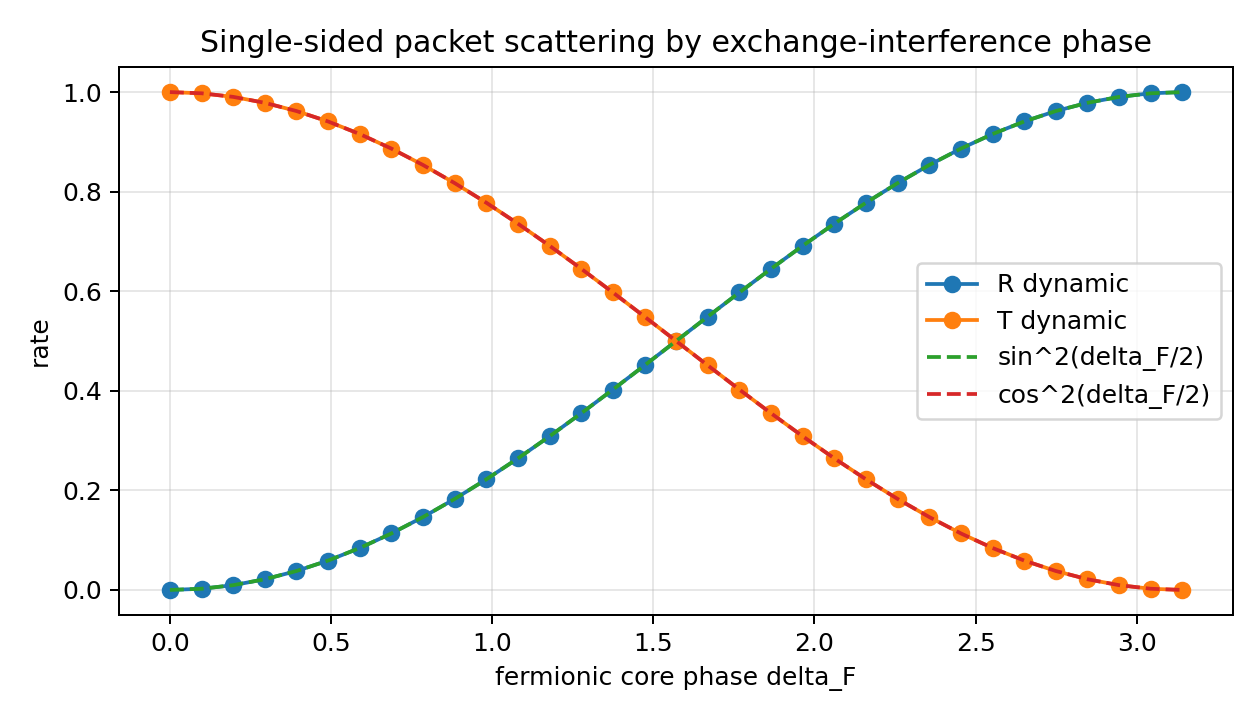
\includegraphics[keepaspectratio,alt={片側入射散乱}]{fermionic_interference_reflection_result_v1/fermionic_interference_single_sided_scattering_v1.png}}

\subsubsection{10.3
交換干渉節}\label{103-ux4ea4ux63dbux5e72ux6e09ux7bc0}

{\def\LTcaptype{none} % do not increment counter
\begin{longtable}[]{@{}lr@{}}
\toprule\noalign{}
量 & 値 \\
\midrule\noalign{}
\endhead
\bottomrule\noalign{}
\endlastfoot
\texttt{Delta\_F=pi} 対角相対ノルム & \texttt{7.4987989133092880e-33} \\
位相掃引最大誤差 & \texttt{8.8817841970012523e-16} \\
交換あり \texttt{Delta\_F=pi} & \texttt{7.4987989133092880e-33} \\
交換なし \texttt{Delta\_F=pi} & \texttt{4.9999999999999994e-01} \\
\end{longtable}
}

\pandocbounded{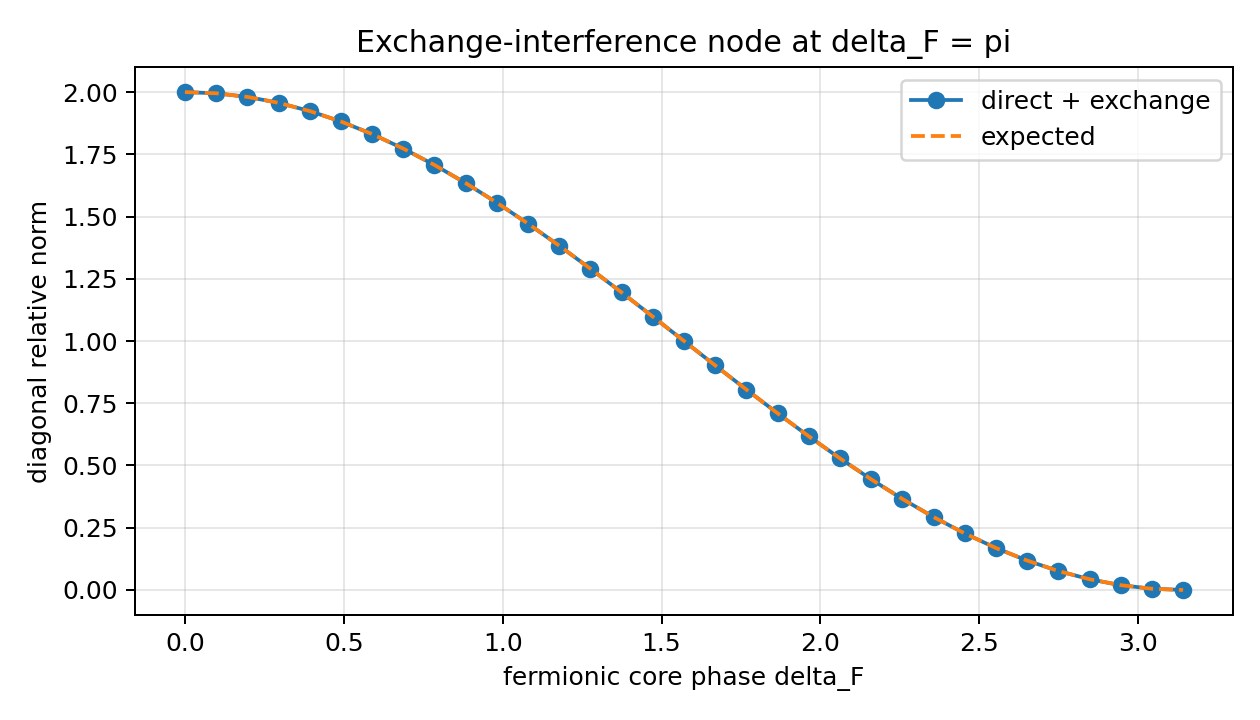
\includegraphics[keepaspectratio,alt={交換干渉位相掃引}]{fermionic_interference_reflection_result_v1/fermionic_interference_phase_sweep_v1.png}}

\subsubsection{10.4
奇関数節の補助読出し}\label{104-ux5947ux95a2ux6570ux7bc0ux306eux88dcux52a9ux8aadux51faux3057}

片側入射散乱とは別に、逆相核に対応する奇関数節をあらかじめ持つ相対位相波も補助的に確認した。この確認は主判定ではなく、節を持つ波が半線読出しで反射波として読めることの補助確認である。

{\def\LTcaptype{none} % do not increment counter
\begin{longtable}[]{@{}lr@{}}
\toprule\noalign{}
量 & 値 \\
\midrule\noalign{}
\endhead
\bottomrule\noalign{}
\endlastfoot
単一自由波束の最終左確率 & \texttt{8.6915330692793126e-05} \\
奇関数節の最終左確率 & \texttt{4.9999999999999994e-01} \\
奇関数節の最終左電流 & \texttt{-1.1980224685843772e+00} \\
奇関数節の最大節振幅 & \texttt{3.0038078125523204e-17} \\
奇関数節の最大節電流 & \texttt{3.7549762132062191e-17} \\
\end{longtable}
}

\pandocbounded{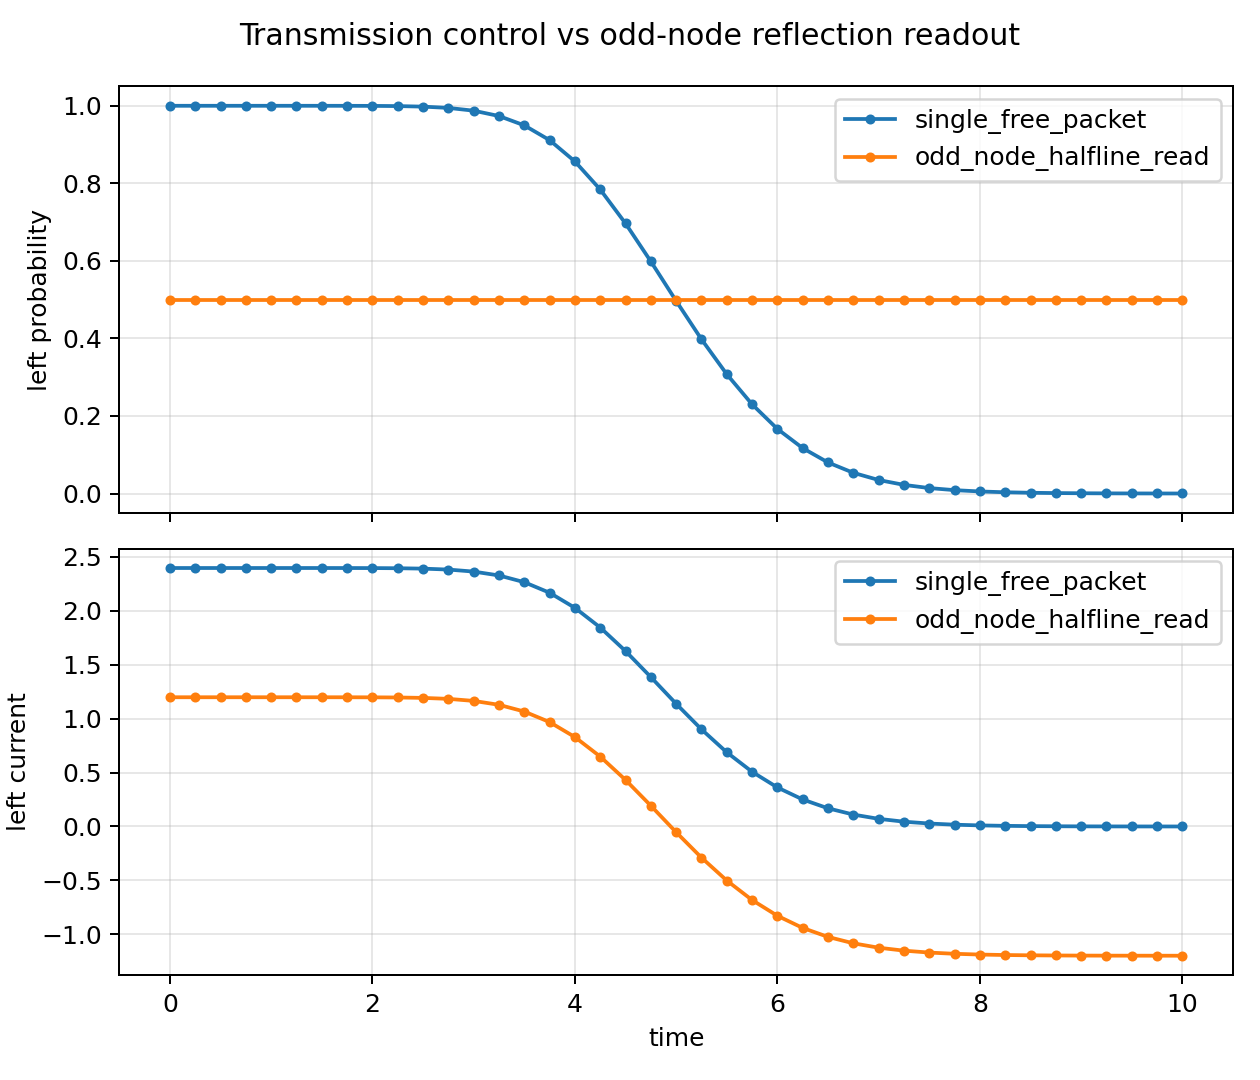
\includegraphics[keepaspectratio,alt={相対時間発展}]{fermionic_interference_reflection_result_v1/fermionic_interference_relative_dynamics_v1.png}}

\subsubsection{10.5
識別振動読出し}\label{105-ux8b58ux5225ux632fux52d5ux8aadux51faux3057}

{\def\LTcaptype{none} % do not increment counter
\begin{longtable}[]{@{}lr@{}}
\toprule\noalign{}
項目 & 結果 \\
\midrule\noalign{}
\endhead
\bottomrule\noalign{}
\endlastfoot
A の検出モード & \texttt{1} \\
B の検出モード & \texttt{2} \\
A ターゲット振幅 & \texttt{1.0000000000000000e+00} \\
B ターゲット振幅 & \texttt{1.0000000000000000e+00} \\
\end{longtable}
}

識別振動 \texttt{η}
は、反射生成チャネルではなく、保存される読出しチャネルとして扱った。異なる
\texttt{m\_A,m\_B}
を交換消去チャネルへ直接混ぜると、空間重なり節が壊れる。したがって、反射はフェルミオン的逆相核の交換干渉で生成し、A/B
の識別は \texttt{η} 相関で読出す。

\subsubsection{10.6
可逆性と補償付き二乗閉鎖}\label{106-ux53efux9006ux6027ux3068ux88dcux511fux4ed8ux304dux4e8cux4e57ux9589ux9396}

局所交換干渉写像を二回適用し、波形が元へ戻るかを測定した。また、各サンプル係数
\texttt{x\_n} に補償対 \texttt{i\ x\_n}
を付け、主要段階で補償付き二乗閉鎖を評価した。

{\def\LTcaptype{none} % do not increment counter
\begin{longtable}[]{@{}lr@{}}
\toprule\noalign{}
量 & 値 \\
\midrule\noalign{}
\endhead
\bottomrule\noalign{}
\endlastfoot
\texttt{U(pi)\^{}2} 相対誤差 & \texttt{4.8214412843789535e-11} \\
\texttt{U(delta)U(-delta)} 最大相対誤差 &
\texttt{1.4547631339456792e-16} \\
補償付き二乗閉鎖 最大残差 & \texttt{1.2143074258005000e-17} \\
\end{longtable}
}

\texttt{U(pi)\^{}2}
の誤差は、局所窓と補間を含む実装上の数値誤差であり、判定閾値
\texttt{1e-10} 内に収まった。\texttt{U(delta)U(-delta)}
は位相掃引全体で機械精度範囲に収まった。

\subsubsection{10.7 AB/C
相互作用セル差し替え}\label{107-abc-ux76f8ux4e92ux4f5cux7528ux30bbux30ebux5deeux3057ux66ffux3048}

前回の AB/C 完全弾性衝突シミュレーションで用いていたセル内の直接
\texttt{q} 反転を使わず、局所交換干渉写像から得た反射率 \texttt{R}
と通過率 \texttt{T} により、

\begin{Shaded}
\begin{Highlighting}[]
\NormalTok{q\_out = q\_in * (T {-} R)}
\end{Highlighting}
\end{Shaded}

として進行方向読出し量を生成した。\texttt{Δ\_F=π} では
\texttt{R=1.0000000000000002}, \texttt{T=1.7939211291143336e-19}
が用いられた。

{\def\LTcaptype{none} % do not increment counter
\begin{longtable}[]{@{}lr@{}}
\toprule\noalign{}
項目 & 値 \\
\midrule\noalign{}
\endhead
\bottomrule\noalign{}
\endlastfoot
AB/C 差し替え成立 & \texttt{true} \\
collision\_cell\_reached & \texttt{true} \\
post\_collision\_completed & \texttt{true} \\
\texttt{q\_A} before/after & \texttt{1.0000000000000000e+00} /
\texttt{-1.0000000000000002e+00} \\
\texttt{q\_B} before/after & \texttt{-1.0000000000000000e+00} /
\texttt{1.0000000000000002e+00} \\
label A initial/final & \texttt{1} / \texttt{1} \\
label B initial/final & \texttt{2} / \texttt{2} \\
\end{longtable}
}

\pandocbounded{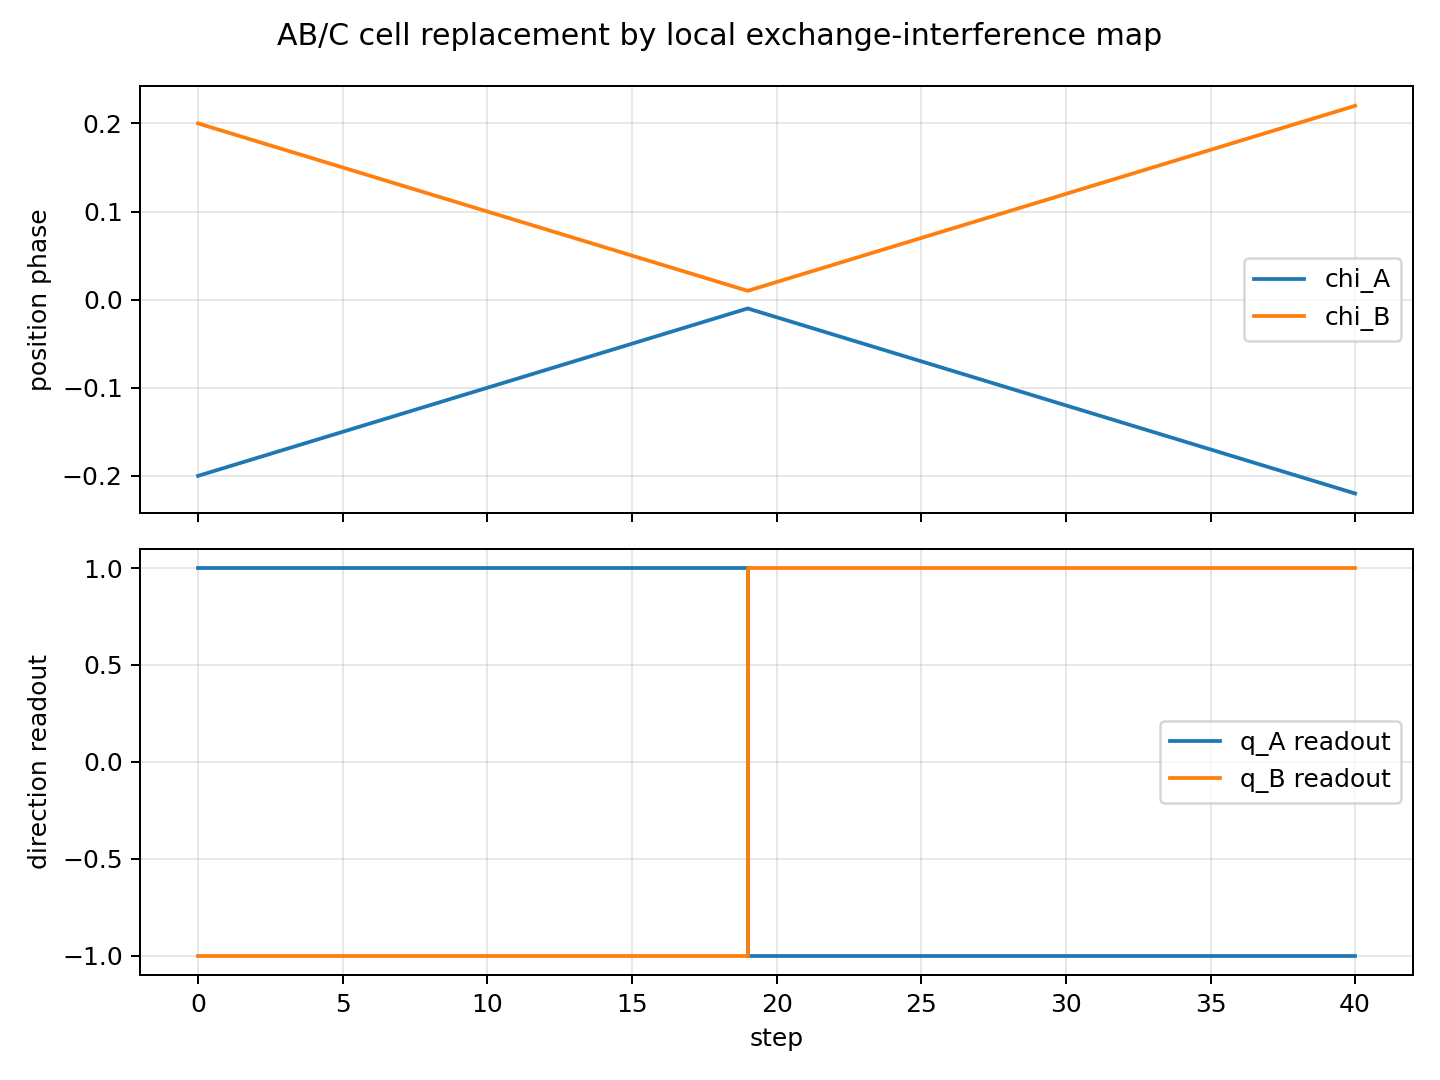
\includegraphics[keepaspectratio,alt={AB/Cセル差し替え}]{fermionic_interference_reflection_result_v1/fermionic_interference_ab_c_replacement_v1.png}}

\begin{center}\rule{0.5\linewidth}{0.5pt}\end{center}

\subsection{11. 評価量}\label{11-ux8a55ux4fa1ux91cf}

\subsubsection{11.1 通過率}\label{111-ux901aux904eux7387}

\[T
=
\frac{I_{\mathrm{trans}}}
{I_{\mathrm{trans}}+I_{\mathrm{refl}}}\]

\subsubsection{11.2 反射率}\label{112-ux53cdux5c04ux7387}

\[R
=
\frac{I_{\mathrm{refl}}}
{I_{\mathrm{trans}}+I_{\mathrm{refl}}}\]

\subsubsection{11.3
識別モード読出し}\label{113-ux8b58ux5225ux30e2ux30fcux30c9ux8aadux51faux3057}

\[O_{P,m}^{(j)}
=
\frac{1}{(2\pi)^3}
\iiint
P
C_{\mathrm{read},P}^{(j)}
e^{-im\eta}
\,d\chi d\tau d\eta\]

\subsubsection{11.4
期待する位相依存性}\label{114-ux671fux5f85ux3059ux308bux4f4dux76f8ux4f9dux5b58ux6027}

理想的な二チャンネル干渉では、

\[R(\Delta_F)
=
\sin^2\frac{\Delta_F}{2}\]

\[T(\Delta_F)
=
\cos^2\frac{\Delta_F}{2}\]

が期待される。

理想的な二チャンネル干渉演算からは、上式が解析的に得られる。数値実験では、これらの値を反射率・通過率として直接代入するのではなく、片側入射波束の自由伝播、局所的な偶奇チャンネル分解、内部位相転写、および再合成を実行し、最終波形から
\texttt{R,T}
を測定する。位相掃引は、実装された局所交換干渉写像が解析的二チャンネル写像と一致することの検証である。

\subsubsection{11.5 閉鎖残差}\label{115-ux9589ux9396ux6b8bux5dee}

\[\mathcal R_{\mathrm{closure}}
=
\left|
\sum_n x_n^2
\right|\]

\subsubsection{11.6 可逆性}\label{116-ux53efux9006ux6027}

反射干渉過程を二回適用したとき、

\[\mathcal U_F^2\approx I\]

となるかを数値的に評価する。

\begin{center}\rule{0.5\linewidth}{0.5pt}\end{center}

\subsection{12. 成功条件}\label{12-ux6210ux529fux6761ux4ef6}

本構成を反射写像の内部生成と判定するため、今回の最小実行では次を要求した。

\begin{enumerate}
\def\labelenumi{\arabic{enumi}.}
\tightlist
\item
  初期状態が左側だけに置かれた単一入射波束である。
\item
  外部の \texttt{q=-q} 命令を使用しない。
\item
  \texttt{Δ\_F=0} で
  \texttt{R\textbackslash{}simeq0,T\textbackslash{}simeq1} となる。
\item
  \texttt{Δ\_F=\textbackslash{}pi/2} で
  \texttt{R\textbackslash{}simeq\ T\textbackslash{}simeq1/2} となる。
\item
  \texttt{Δ\_F=\textbackslash{}pi} で
  \texttt{R\textbackslash{}simeq1,T\textbackslash{}simeq0} となる。
\item
  位相掃引全体で \texttt{R(Δ\_F)=sin\^{}2(Δ\_F/2)},
  \texttt{T(Δ\_F)=cos\^{}2(Δ\_F/2)} が成立する。
\item
  時間発展と相互作用を通じてノルムが保存される。
\item
  \texttt{Δ\_F=π} で完全重なり対角のノルムが数値誤差範囲まで低下する。
\item
  交換経路を削除すると節形成が消える。
\item
  識別振動 \texttt{m\_A,m\_B} が読出しで保存される。
\item
  \texttt{U(π)\^{}2≈I} および \texttt{U(Δ\_F)U(-Δ\_F)≈I} が成り立つ。
\item
  補償付き二乗閉鎖の残差が閾値内に保たれる。
\item
  前回 AB/C
  シミュレーションのセル内方向反転を、\texttt{q\_out=q\_in*(T-R)}
  として局所交換干渉写像から生成できる。
\end{enumerate}

\begin{center}\rule{0.5\linewidth}{0.5pt}\end{center}

\subsection{13. 破綻条件}\label{13-ux7834ux7dbbux6761ux4ef6}

{\def\LTcaptype{none} % do not increment counter
\begin{longtable}[]{@{}ll@{}}
\toprule\noalign{}
破綻条件 & 意味 \\
\midrule\noalign{}
\endhead
\bottomrule\noalign{}
\endlastfoot
節はできるが反射波が生成されない & 通過消去だけで方向反転機構が不足 \\
\texttt{Δ\_F=π} でも通過が残る &
交換経路の振幅整合または位相転写が不完全 \\
反射率を外部正規化しないと1にならない &
干渉だけで完全反射を生成できていない \\
識別振動が交換される & 見かけ上の反射と個体保存を区別できない \\
交換経路なしでも反射する & 別の数値境界条件が反射を作っている可能性 \\
代表振幅が増大する & 干渉再合成の正規化が不適切 \\
\texttt{R+T} が1から外れる & 読出し定義または閉鎖条件の不足 \\
\end{longtable}
}

\begin{center}\rule{0.5\linewidth}{0.5pt}\end{center}

\subsection{14. 考察}\label{14-ux8003ux5bdf}

\subsubsection{14.1
演算の選択は判断ではない}\label{141-ux6f14ux7b97ux306eux9078ux629eux306fux5224ux65adux3067ux306fux306aux3044}

本構成では、局所波が自分自身をフェルミオンと認識して演算を選択するのではない。

\[\Delta_F\]

が交換経路の相対位相として直接現れ、干渉結果を決める。

したがって、演算選択は外部判断ではなく、結合可能な位相チャンネルの選択則である。

\subsubsection{\texorpdfstring{14.2 \texttt{π/2}
の外部調整を必要としない}{14.2 π/2 の外部調整を必要としない}}\label{142-ux3c02-ux306eux5916ux90e8ux8abfux6574ux3092ux5fc5ux8981ux3068ux3057ux306aux3044}

完全反転行列を二状態回転として書けば \texttt{π/2}
が現れるが、本構成ではその積分角を外部から与えない。

直接原因は、

\[1+e^{i\pi}=0\]

による交換二経路の完全消去である。

\subsubsection{14.3
片側入射による反射生成}\label{143-ux7247ux5074ux5165ux5c04ux306bux3088ux308bux53cdux5c04ux751fux6210}

\[\Psi_F(0)=0\]

だけでは、反射生成の確認には足りない。そこで本稿では、最初から奇関数波を置くのではなく、左側から入射する単一波束を初期状態とした。

相互作用前の初期右側確率は、

\begin{Shaded}
\begin{Highlighting}[]
\NormalTok{2.4303500961591473e{-}89}
\end{Highlighting}
\end{Shaded}

であり、反射成分または鏡像成分は初期状態に埋め込まれていない。その上で、自由伝播により相互作用領域へ到達した波束を偶・奇干渉チャンネルへ分解し、内部核位相
\texttt{Δ\_F} だけを奇チャンネルへ転写した。

この処理により、\texttt{Δ\_F=0} では通過率が1へ、\texttt{Δ\_F=π}
では反射率が1へ変換された。したがって、反射は初期条件の鏡像構造ではなく、相互作用領域での局所交換干渉写像から生成された。

\subsubsection{14.4
局所写像方式としての本実装}\label{144-ux5c40ux6240ux5199ux50cfux65b9ux5f0fux3068ux3057ux3066ux306eux672cux5b9fux88c5}

本実装は、相互作用ハミルトニアン \texttt{H\_int(ρ,Δ\_F)}
を連続時間で積分する方式ではない。計算順序は、

\begin{Shaded}
\begin{Highlighting}[]
\NormalTok{片側入射波束の自由伝播}
\NormalTok{→ 相互作用窓内での偶奇チャンネル分解}
\NormalTok{→ 奇チャンネルへの内部核位相 Δ\_F の転写}
\NormalTok{→ 再合成}
\NormalTok{→ 自由伝播後の R,T 読出し}
\end{Highlighting}
\end{Shaded}

である。したがって、本稿で確認したのは、外部の \texttt{q=-q}
命令を、内部逆相核の位相で制御される局所交換干渉写像へ置換できることである。

\begin{center}\rule{0.5\linewidth}{0.5pt}\end{center}

\subsection{15. 結論}\label{15-ux7d50ux8ad6}

本稿では、前論文で有限解像度相互作用セル内の構成規則として与えた方向反転写像を、フェルミオン的内部逆相核と交換二経路の干渉から内部生成する最小機構として実行した。

内部位相差 \texttt{Δ\_F}
を直接経路と交換経路の相対位相として転写すると、純粋フェルミオン的条件
\texttt{Δ\_F=π}
において、完全重なり点の波形は厳密にゼロとなる。実行結果では、\texttt{Δ\_F=π}
の対角相対ノルムは \texttt{7.4987989133092880e-33}
となり、交換経路を除去した場合には \texttt{4.9999999999999994e-01}
が残った。したがって、節形成は交換二経路干渉によって生成された。

片側入射波束を用いた局所交換干渉散乱では、\texttt{Δ\_F=0} に対して反射率
\texttt{1.8261693781071190e-19}、通過率 \texttt{1.0000000000000002}
が得られた。\texttt{Δ\_F=π/2} では反射率・通過率ともに
\texttt{0.5}、\texttt{Δ\_F=π} では反射率
\texttt{1.0000000000000002}、通過率 \texttt{1.7939211291143336e-19}
が得られた。位相掃引全体で \texttt{R(Δ\_F)=sin\^{}2(Δ\_F/2)},
\texttt{T(Δ\_F)=cos\^{}2(Δ\_F/2)} が最大誤差
\texttt{5.551115123125783e-16} で成立し、ノルム最大誤差は
\texttt{6.661338147750939e-16} であった。

局所交換干渉写像の可逆性については、\texttt{U(π)\^{}2} の相対誤差が
\texttt{4.8214412843789535e-11}、\texttt{U(Δ\_F)U(-Δ\_F)}
の最大相対誤差が \texttt{1.4547631339456792e-16}
であった。補償付き二乗閉鎖の最大残差は \texttt{1.2143074258005e-17}
であった。

さらに、前回の AB/C
完全弾性衝突シミュレーションの相互作用セルにおいて、直接的な \texttt{q}
反転命令を使わず、局所交換干渉写像から得た \texttt{R,T} により
\texttt{q\_out=q\_in*(T-R)}
として進行方向読出し量を生成した。この差し替え統合テストでは、\texttt{q\_A}
は \texttt{1.0} から \texttt{-1.0000000000000002} へ、\texttt{q\_B} は
\texttt{-1.0} から \texttt{1.0000000000000002} へ変換され、識別振動
\texttt{m\_A=1}, \texttt{m\_B=2} は初期・最終読出しで保存された。

以上により、外部条件分岐、人工的な \texttt{q=-q}
命令、鏡像初期条件、反射境界条件を使わず、内部逆相核、局在波重なり、交換経路、偶・奇干渉チャンネル、局所位相転写、および識別振動読出しから、完全弾性反射に相当する方向反転出力が、片側入射波束の自由伝播と局所交換干渉写像によって生成された。

\begin{center}\rule{0.5\linewidth}{0.5pt}\end{center}

\section{付録A.
実行済みプログラムと出力}\label{ux4ed8ux9332a-ux5b9fux884cux6e08ux307fux30d7ux30edux30b0ux30e9ux30e0ux3068ux51faux529b}

今回の実行に用いたプログラムは次である。

\begin{Shaded}
\begin{Highlighting}[]
\NormalTok{run\_fermionic\_interference\_reflection\_v1.py}
\end{Highlighting}
\end{Shaded}

出力ディレクトリは次である。

\begin{Shaded}
\begin{Highlighting}[]
\NormalTok{fermionic\_interference\_reflection\_result\_v1/}
\end{Highlighting}
\end{Shaded}

主要出力は次である。

{\def\LTcaptype{none} % do not increment counter
\begin{longtable}[]{@{}ll@{}}
\toprule\noalign{}
種類 & ファイル \\
\midrule\noalign{}
\endhead
\bottomrule\noalign{}
\endlastfoot
実行レポート &
\href{fermionic_interference_reflection_result_v1/fermionic_interference_reflection_report_v1.md}{fermionic\_interference\_reflection\_report\_v1.md} \\
結果 JSON &
\href{fermionic_interference_reflection_result_v1/fermionic_interference_reflection_result_v1.json}{fermionic\_interference\_reflection\_result\_v1.json} \\
位相掃引 CSV &
\href{fermionic_interference_reflection_result_v1/fermionic_interference_phase_sweep_v1.csv}{fermionic\_interference\_phase\_sweep\_v1.csv} \\
相対時間発展 CSV &
\href{fermionic_interference_reflection_result_v1/fermionic_interference_relative_dynamics_v1.csv}{fermionic\_interference\_relative\_dynamics\_v1.csv} \\
片側入射散乱 CSV &
\href{fermionic_interference_reflection_result_v1/fermionic_interference_single_sided_scattering_v1.csv}{fermionic\_interference\_single\_sided\_scattering\_v1.csv} \\
可逆性 CSV &
\href{fermionic_interference_reflection_result_v1/fermionic_interference_reversibility_sweep_v1.csv}{fermionic\_interference\_reversibility\_sweep\_v1.csv} \\
AB/C 差し替え CSV &
\href{fermionic_interference_reflection_result_v1/fermionic_interference_ab_c_replacement_timeline_v1.csv}{fermionic\_interference\_ab\_c\_replacement\_timeline\_v1.csv} \\
交換干渉節の図 &
\href{fermionic_interference_reflection_result_v1/fermionic_interference_phase_sweep_v1.png}{fermionic\_interference\_phase\_sweep\_v1.png} \\
相対時間発展の図 &
\href{fermionic_interference_reflection_result_v1/fermionic_interference_relative_dynamics_v1.png}{fermionic\_interference\_relative\_dynamics\_v1.png} \\
片側入射散乱の図 &
\href{fermionic_interference_reflection_result_v1/fermionic_interference_single_sided_scattering_v1.png}{fermionic\_interference\_single\_sided\_scattering\_v1.png} \\
AB/C 差し替えの図 &
\href{fermionic_interference_reflection_result_v1/fermionic_interference_ab_c_replacement_v1.png}{fermionic\_interference\_ab\_c\_replacement\_v1.png} \\
\end{longtable}
}

実行コマンドは次である。

\begin{Shaded}
\begin{Highlighting}[]
\NormalTok{python3 run\_fermionic\_interference\_reflection\_v1.py}
\end{Highlighting}
\end{Shaded}

この実装では、外部方向反転代入は使用していない。結果 JSON
の判定は次である。

\begin{Shaded}
\begin{Highlighting}[]
\NormalTok{external\_q\_flip\_used: false}
\NormalTok{single\_sided\_initial\_packet: true}
\NormalTok{dynamic\_transmission\_at\_zero: true}
\NormalTok{dynamic\_half\_phase\_split: true}
\NormalTok{dynamic\_reflection\_at\_pi: true}
\NormalTok{dynamic\_phase\_sweep\_matches\_expected: true}
\NormalTok{dynamic\_norm\_preserved: true}
\NormalTok{static\_node\_at\_pi: true}
\NormalTok{phase\_sweep\_matches\_expected: true}
\NormalTok{exchange\_path\_required: true}
\NormalTok{label\_mode\_preserved\_A: true}
\NormalTok{label\_mode\_preserved\_B: true}
\NormalTok{pi\_twice\_reversible: true}
\NormalTok{inverse\_sweep\_reversible: true}
\NormalTok{compensated\_square\_closure\_preserved: true}
\NormalTok{ab\_c\_replacement\_valid: true}
\NormalTok{mechanism\_valid\_minimal: true}
\end{Highlighting}
\end{Shaded}

\begin{center}\rule{0.5\linewidth}{0.5pt}\end{center}

\section{付録B.
旧雛形の扱い}\label{ux4ed8ux9332b-ux65e7ux96dbux5f62ux306eux6271ux3044}

ChatGPT
が作成した旧プログラム雛形は、今回の判定には使用しない。理由は、旧雛形の
\texttt{exchange\_coordinates()}
が一粒子波形の反転であり、二粒子の直接経路 \texttt{P\_A(1)P\_B(2)}
と交換経路 \texttt{P\_A(2)P\_B(1)} を明示構成していなかったためである。

今回の実行では、次を満たす実装へ置き換えた。

\begin{enumerate}
\def\labelenumi{\arabic{enumi}.}
\tightlist
\item
  完全重なり対角で直接経路と交換経路を明示的に比較する。
\item
  \texttt{Delta\_F=pi} で対角ノルムが消えることを測定する。
\item
  交換経路を除去すると節が消えることを測定する。
\item
  片側入射波束を走らせ、\texttt{Δ\_F=0,\textbackslash{}pi/2,\textbackslash{}pi}
  および全位相掃引で \texttt{R,T} を測定する。
\item
  単一自由波束と奇関数節の半線読出しを補助確認として残す。
\item
  \texttt{eta}
  識別振動は反射生成チャネルから分け、保存される読出しチャネルとして確認する。
\item
  外部方向反転命令 \texttt{q=-q} を使用しない。
\end{enumerate}

この置き換えにより、旧雛形は設計メモとしてのみ残し、論文の実行根拠は付録Aの実行済みプログラムと出力に一本化する。

\end{document}
